\chapter{常用半导体器件}
半导体器件是构成电子电路的基本元件。为了能够更好地运用这些器件,需要了解各半导体器件的基本特性。

\section{基础知识}
构成半导体器件的基本材料是半导体。因此,为了理解半导体器件的工作特性,需要先了解半导体的基本特性。

\subsection{本征半导体}

\subsubsection{一、半导体}
\textbf{半导体}\index{B!半导体}是指导电能力介于导体和绝缘体之间的材料;在此基础上,纯净的具有完整晶体结构的半导体称为\textbf{本征半导体}\index{B!本征半导体}。常见的半导体材料有硅、锗、砷化镓等等,其中硅的结构如图\ref{硅的结构示意图}所示。

\begin{figure}[htb]
    \centering
        \subcaptionbox{硅的二维结构示意图\cite{康华光}\label{硅的二维结构}}
        {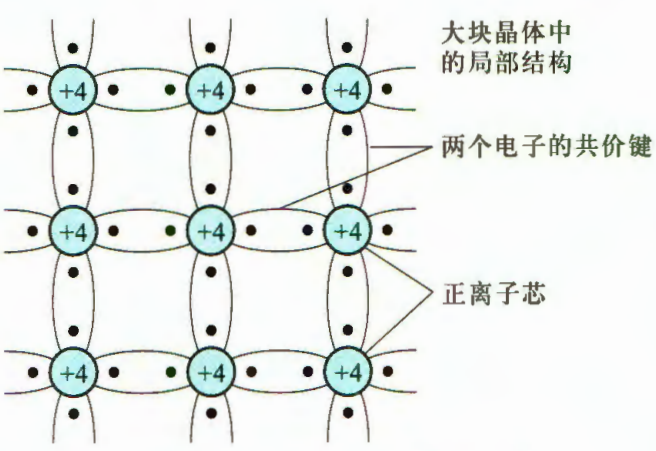
\includegraphics[width=0.4\textwidth]{pic/硅的二维结构.png}}\qquad
        \subcaptionbox{硅的三维结构示意图\cite{阎守胜}\label{硅的三维结构}}
        {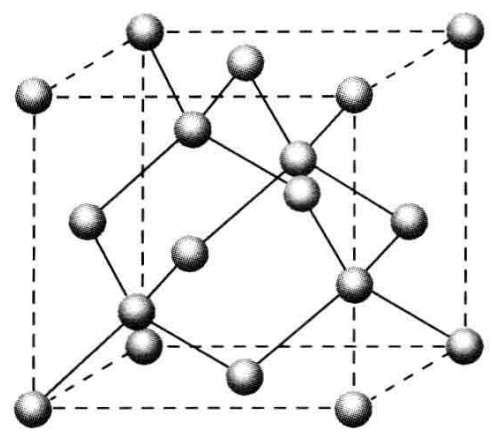
\includegraphics[width=0.3\textwidth]{pic/硅的三维结构.png}}
    \caption{硅的结构示意图\label{硅的结构示意图}}
\end{figure}

\subsubsection{二、本征激发}
半导体中能够自由移动的带电粒子称为\textbf{载流子}\index{Z!载流子};在室温下,部分价电子会挣脱共价键的束缚,成为\textbf{自由电子}\index{Z!自由电子},此时共价键中留下的空位称作\textbf{空穴}\index{K!空穴},这种现象称作\textbf{本征激发}\index{B!本征激发}。可以看到,本征半导体中有两种载流子——自由电子和空穴。当自由电子与空穴相遇就会填补空穴,这种现象称作\textbf{复合}\index{F!复合}。

总体上,温度越高,载流子浓度越大。因为温度越高热运动越剧烈,本征激发越多,随后复合的概率随之上升,最后本征激发和复合重新达到\textbf{动态平衡}。

\subsection{杂质半导体}
在室温下,本征激发产生的载流子浓度较低,且与温度密切相关,因此人们选择了掺杂来解决上述问题。

通过扩散工艺,在本征半导体中掺入少量杂质元素,就成为\textbf{杂质半导体}\index{Z!杂质半导体},如图\ref{P型半导体与N型半导体}所示。

若掺入五价元素(如磷),就成为\textbf{N型半导体}\index{N!N型半导体}(Negative),其中五价元素称为\textbf{施主杂质}\index{S!施主杂质},其中自由电子较多,称为\textbf{多子}\index{D!多子},而空穴较少,称为\textbf{少子}\index{S!少子}。若掺入三价元素(如硼),就成为\textbf{P型半导体}\index{P!P型半导体}(Positive),其中三价元素称为\textbf{受主杂质}\index{S!受主杂质}。

\begin{figure}[htb]
    \centering
    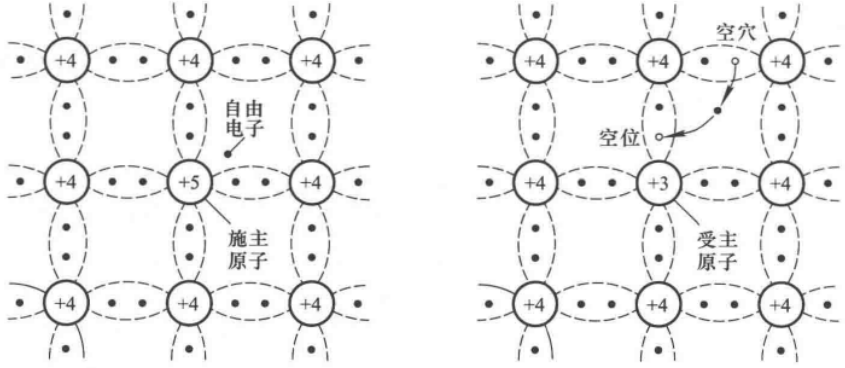
\includegraphics[width=0.8\linewidth]{pic/P型半导体与N型半导体.png}
    \caption{P型半导体与N型半导体\cite{华成英}\label{P型半导体与N型半导体}}
\end{figure}

注意,掺入P(磷)元素的本征半导体为N型半导体。

\subsection{PN结}
将P型半导体与N型半导体制作在同一块硅片上,在交界面处就形成了\textbf{PN结}\index{P!PN结}。\textbf{PN结具有单向导电性}。

\subsubsection{一、PN结的形成}
PN结的形成来源于\textbf{扩散运动}\index{K!扩散运动}和\textbf{漂移运动}\index{P!漂移运动}。其实漂移和扩散只不过是载流子运动的分解,分成了定向的运动和无规则的运动。

1.扩散运动:物质从浓度高的地方向浓度低的地方运动;

2.漂移运动:在电场的作用下载流子的运动。

\textbf{多子扩散}使得交界面处的电⼦和空⽳复合,形成\textbf{空间电荷区(PN结、耗尽区)}\index{K!空间电荷区}\index{H!耗尽区},进而此时内部形成由N区指向P区的内电场,促进\textbf{少子漂移},最终二者达到动态平衡。

当P区和N区杂质浓度不同时,称为\textbf{不对称PN结}\index{B!不对称PN结}。

\subsubsection{二、单向导电性}
1.外加正向电压时导通:

当P区电位高于N区电位时,称所加电压为\textbf{正向电压}\index{Z!正向电压},也称为\textbf{PN结正向偏置}。外加的正向电压削弱了内电场作用,使得少子漂移减少,多子扩散增加,耗尽层逐渐变窄。此时回路电流基本取决于扩散电流,称为正向电流$I_\mathrm{F}$,PN结表现为一个很小的电阻,也称为PN结正向导通。

2.外加反向电压时截止:

当N区电位高于P区电位时,称所加电压为\textbf{反向电压}\index{F!反向电压},也称为\textbf{PN结反向偏置}。此时耗尽区加宽,反向电流趋于0,但少子漂移运动增强,形成微弱的漂移电流,称为反向电流$I_\mathrm{R}$。

\subsubsection{三、PN结的伏安特性曲线}

\begin{figure}[htb]
    \centering
    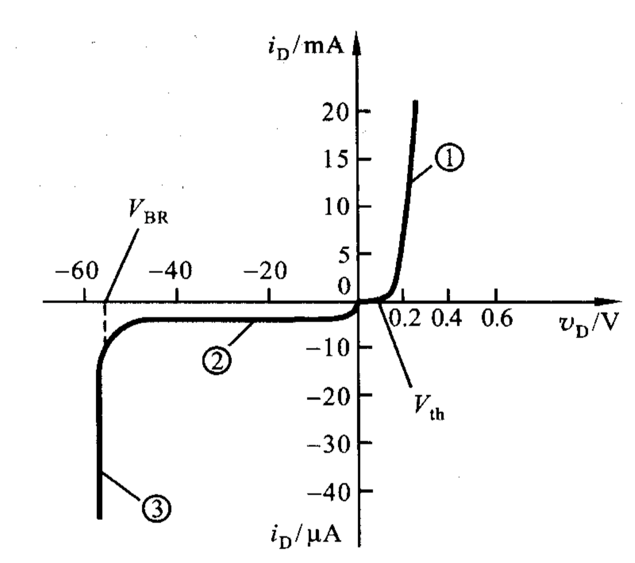
\includegraphics[width=0.5\linewidth]{pic/锗PN结的伏安特性曲线.png}
    \caption{PN结的伏安特性曲线(图片来源:曹平老师PPT-ch3)\label{PN结的伏安特性曲线}}
\end{figure}

不考虑击穿时,PN结两端的电压$v_\mathrm{D}$和电流$i_\mathrm{D}$的关系为

\begin{equation}
    i_{\mathrm{D}}=I_{\mathrm{S}}(\me^{\frac{v_\mathrm{D}}{nV_\mathrm{T}}}-1),
\end{equation}

通常,$n=1$,常温下\textbf{电压当量}\index{D!电压当量}$V_\mathrm{T}=\qty{26}{mV}$,$I_{\mathrm{S}}$为\textbf{反向饱和电流}\index{F!反向饱和电流}。

\textbf{PN结的伏安特性曲线,如图\ref{PN结的伏安特性曲线}所示。}

\subsubsection{四、PN结的反向击穿}
当反向电压大到一定数值时,反向电流突然增加,这种现象称为\textbf{反向击穿}。反向击穿电压记为$V_\mathrm{BR}$。PN结的击穿主要有以下两种原因:

1.\textbf{雪崩击穿}\index{X!雪崩击穿}(不可控):

掺杂浓度较低时,耗尽层较宽,高速少子将共价键中价电子撞出并形成电子-空穴对(\textbf{碰撞电离}),新的电子和空穴又撞出其他价电子,载流子雪崩式增加(\textbf{倍增效应});

2.\textbf{齐纳击穿}\index{Q!齐纳击穿}(可控——稳压二极管):

掺杂浓度较高时,耗尽层较窄,场强极大使得价电子直接从共价键中被拉出来,变成自由电子。

以上二者均可逆,但功率过高会发生不可逆的\textbf{热击穿}\index{R!热击穿}。

\subsubsection{五、PN结的电容特性}
一个器件的电压变化,储存的电荷量跟着变化,就会反映出电容特性。一般在高频丝滑才会考虑其电容特性。

1.\textbf{扩散电容}\index{K!扩散电容}:

穿过PN结未被复合的载流子称为\textbf{超量载流子}。在PN结附近,N区有空穴的积累,P区也有电子的积累,可以视为电荷存储到PN结邻域,外施电压的变化会导致PN结邻区存储电荷的变化,等效电容记作$C_\mathrm{D}$;

2.\textbf{势垒电容}\index{S!势垒电容}:

反偏时,离子在PN结交界处聚集形成的势垒区,是积累空间电荷的区域。电压改变时,引起空间电荷区大小变化,导致积累的空间电荷的改变,等效电容记作$C_\mathrm{B}$。

\section{二极管}
人们在发现PN结的特性后,将其包裹起来并引出两个电极,就形成了\textbf{二极管}\index{E!二极管}。
\subsection{二极管的结构}
二极管分为点接触型、面接触型、平面型。平面型二极管的结构示意图及二极管的代表符号如图\ref{二极管的结构及符号}所示。

\begin{figure}[htb]
    \centering
        \subcaptionbox{二极管的结构及符号\cite{康华光}\label{二极管的结构及符号}}
        {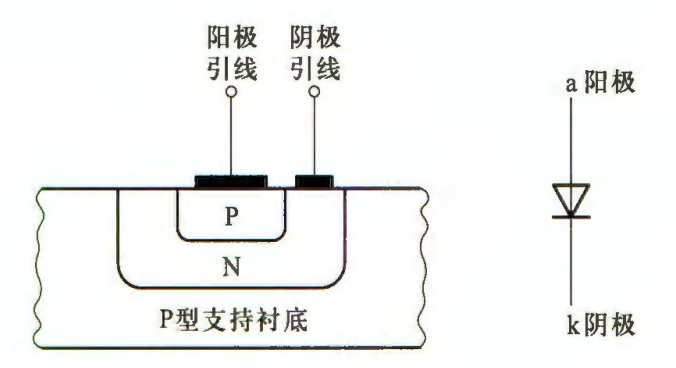
\includegraphics[width=0.4\textwidth]{pic/半导体二极管的结构及符号.png}}\qquad
        \subcaptionbox{齐纳二极管的符号\cite{康华光}\label{齐纳二极管的符号}}
        {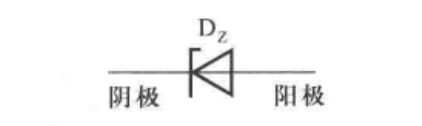
\includegraphics[width=0.3\textwidth]{pic/齐纳二极管的符号.png}}
        \caption{BJT的结构和符号\label{111}}
\end{figure}

齐纳二极管是一种面接触型晶体二极管,很容易形成强电场,符号如图\ref{齐纳二极管的符号}所示。齐纳二极管主要利用齐纳击穿在反向击穿特性$V_{\mathrm{Z}}$附近稳压,在电路中往往只会反接。

\subsection{二极管的伏安特性曲线及主要参数}

二极管的伏安特性和PN结的伏安特性基本相同。

\subsubsection{一、正向特性}

硅管的\textbf{门坎电压(死区电压)}\index{M!门坎槛电压}$V_{\mathrm{th}}$约为$\qty{0.5}{V}$;锗管的$V_{\mathrm{th}}$约为$\qty{0.1}{V}$。

\subsubsection{二、反向特性}
由于少数载流子的数目较少,所以反向电流很小,硅管的反向电流比锗管小得多。反向击穿特性则类似PN结。

\subsection{二极管基本电路及分析方法}
分析非线性电路的基本思想之一就是线性化,进而使用线性电路的分析方法。

\subsubsection{一、大信号模型}
1.\textbf{理想模型}:\index{L!理想模型}理想模型简单好用,但是比较粗糙,参考图\ref{二极管的三种等效模型}(a)。

2.\textbf{恒压降模型}:\index{H!恒压降模型}恒压降模型在⼆极管电路的分析中非常常用,参考图\ref{二极管的三种等效模型}(b)。硅管的正向导通压降约为$\qty{0.7}{V}$;锗管约为$\qty{0.2}{V}$(锗原子半径大,对外层电子束缚小,更易脱离共价键,导通电压低)。

3.\textbf{折线模型}:\index{Z!折线模型}折线模型考虑了动态电阻,但是略复杂,参考图\ref{二极管的三种等效模型}(c)。

\begin{figure}[htb]
    \centering
    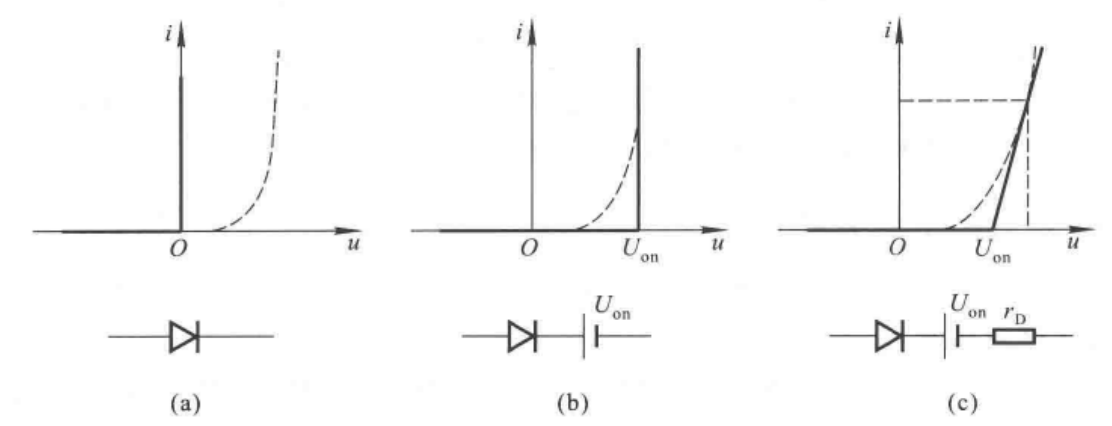
\includegraphics[width=0.8\linewidth]{pic/二极管的三种等效模型.png}
    \caption{二极管的三种等效模型\cite{华成英}\label{二极管的三种等效模型}}
\end{figure}

应用电路:整流电路、开关电路、限幅电路、钳位电路。注意模型和实际元件之间的区别。

二极管工作状态的分析:\textbf{假定全部二极管截止},然后计算每个二极管两端的电压是否大于导通电压。电压大的优先导通,然后再假设剩下的截止,重复上述分析,直到判定完所有二极管的工作状态。

\subsubsection{二、小信号模型}\index{X!小信号模型}
以上三个模型反映了二极管全部特性(除了反向击穿部分),可用于分析工作电压在较大范围内变化的情况,也称作\textbf{大信号模型}\index{D!大信号模型}。当仅仅考虑电压或者电流小幅波动时所建立的模型称为\textbf{小信号模型}。

\begin{figure}[htb]
    \centering
    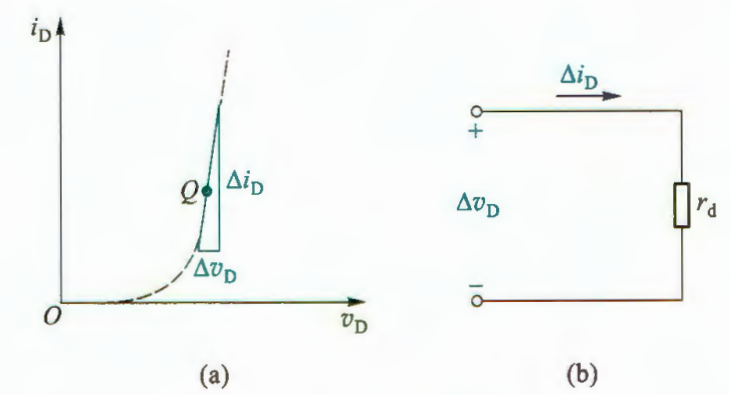
\includegraphics[width=0.6\linewidth]{pic/二极管的小信号模型.png}
    \caption{二极管的小信号模型\cite{康华光}\label{二极管的小信号模型}}
\end{figure}

小信号模型基本分析步骤将会在第二章详细讲解,此处仅做概述。

当电路中仅有直流信号时,称做\textbf{静态}\index{J!静态},$U-I$图上对应的点称作\textbf{静态工作点(Q点)}\index{J!静态工作点}。

二极管的小信号模型——\textbf{微变电阻}\index{W!微变电阻}$r_\mathrm{d}=\frac{V_\mathrm{T}}{I_\mathrm{D}}$,其中$V_\mathrm{T}$为电压当量,$I_\mathrm{D}$为Q点电流。

\section{双极结型三极管(BJT)}\index{S!双极结型三极管}
将两个二极管背靠背拼接起来,就成为了一个三极管。三极管分主要为双极结型三极管(BJT)和场效应三极管(FET)两种。虽然如今广泛应用的三极管主要是MOSFET,但BJT在个别领域也有其优势。由于本课程更侧重于BJT的使用,因此首先讲解BJT。

\textbf{双极结型晶体管(Bipolar Junction Transistor, BJT)}\index{S!双极结型晶体管},又称为半导体三极管或晶体管。其中\textbf{双极型器件}\index{S!双极型器件}是指由电子和空穴两种载流子都参与导电的半导体器件。

\subsection{结构及类型}
\subsubsection{一、结构:三个区域、三个电极、两个PN结}
BJT的结构如图\ref{集成电路中典型NPN型BJT的截面图}所示,可以看到三个区域的一些基本特点:

1.\textbf{发射区/发射极}\index{F!发射区}\index{F!发射极}e(emitter):需要发射载流子,因此掺杂浓度最高,和基区形成\textbf{发射结};

2.\textbf{集电区/集电极}\index{J!集电区}\index{J!集电极}c(collector):需要收集载流子,因此面积最大且掺杂浓度较低,和基区形成\textbf{集电结};

3.\textbf{基区/基极}\index{J!基区}\index{J!基极}b(base):很薄且杂质浓度低,起到控制作用。

\begin{figure}[htb]
    \centering
        \subcaptionbox{集成电路中典型NPN型BJT的截面图\cite{康华光}\label{集成电路中典型NPN型BJT的截面图}}
        {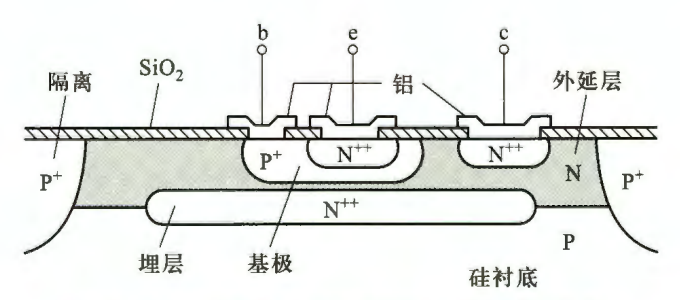
\includegraphics[width=0.68\textwidth]{pic/集成电路中典型NPN型BJT的截面图.png}}\qquad
        \subcaptionbox{BJT的符号\cite{华成英}\label{BJT的符号}}
        {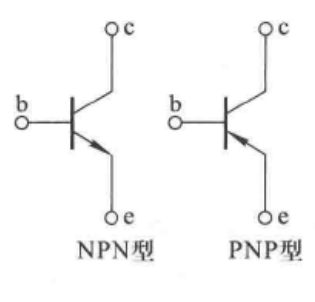
\includegraphics[width=0.28\textwidth]{pic/BJT的符号.png}}
        \caption{BJT的结构和符号\label{BJT的结构和符号}}
\end{figure}

\subsubsection{二、类型}
BJT分为PNP型和NPN型,如图\ref{BJT的符号}所示。注意箭头在基极b和发射极e之间,方向为P指向N。

除非特殊声明,本手册之后所有的BJT均考虑为NPN型。

\subsection{BJT的电流放大作用}
放大是对模拟信号最基本的处理,而三极管是放大电路的核心,它能够控制能量的转换,使微小信号不失真地放大输出。本手册第二章将会专门讨论放大相关的内容。

BJT的放大作用主要体现体现在小的基极电流可以控制大的集电极电流——\textbf{电流控制电流源}。

\subsubsection{一、内部载流子的运动}
\begin{figure}[htb]
	\centering
	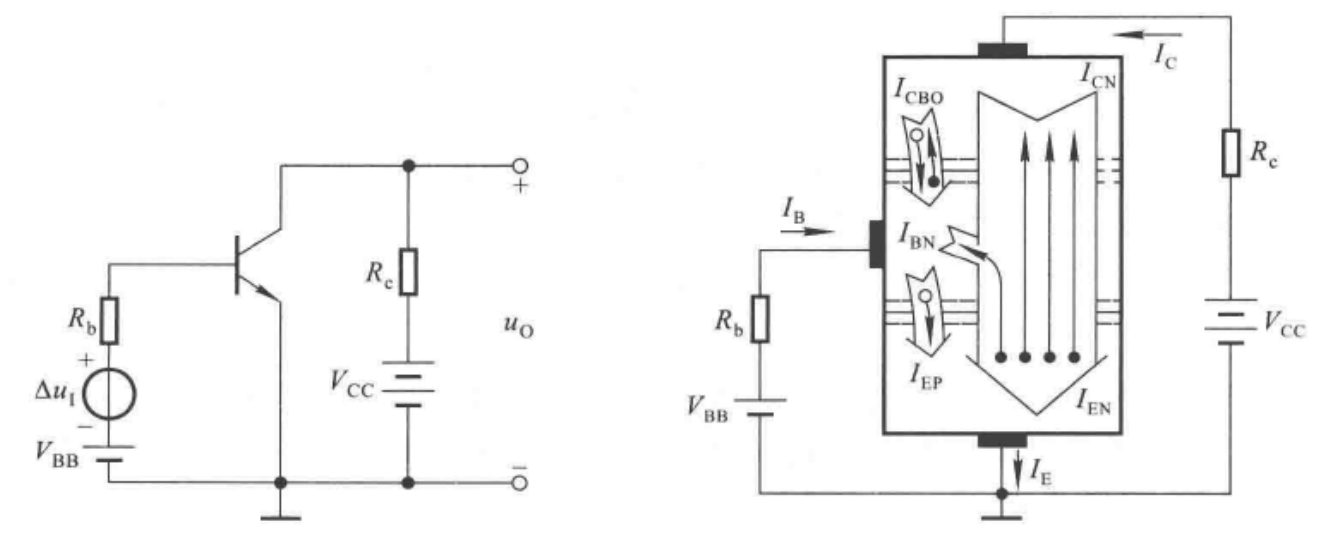
\includegraphics[width=0.8\linewidth]{pic/BJT原理.png}
	\caption{BJT放大的基本原理\cite{华成英}\label{BJT放大}}
\end{figure}

1.发射结正偏:发射区有大量自由电子向基区\underline{扩散},同时基区有少量空穴向发射区\underline{扩散},形成$I_{\mathrm{EN}}$和$I_{\mathrm{EP}}$。由于两个区域掺杂浓度不同,$I_{\mathrm{EN}}\gg I_{\mathrm{EP}}$。扩散运动形成发射极电流$I_{\mathrm{E}}$。

2.基区:由于基区薄且掺杂浓度低,扩散到基区的电子只有极少部分与空穴复合,其余均到达集电极。由于外部电源$V_{\mathrm{BB}}$的存在,自由电子被不断抽走,使得基区空穴浓度保持不变,因此发射区扩散到基区的电子和基区空穴源源不断地复合。这样不断地复合和产生,宏观上形成基极电流$I_{\mathrm{B}}$,而向集电结\underline{漂移}的电子形成$I_{\mathrm{CN}}$。

注意,BJT工作在放大状态的时候,复合的比例是固定的,因此有了“放大倍数”的概念。

3.集电结反偏:由于集电结面积大且反向偏置,它尽可能地在收集从发射区过来的电子,保证从发射区到基区浓度梯度的稳定。当反向偏置到达一定程度后,收集电子能力和偏置电压无关。

\subsubsection{二、常用参数}
由基尔霍夫电流定律可以得到$I_{\mathrm{E}}=I_{\mathrm{B}}+I_{\mathrm{C}}$,其他参数如下:

1.(共射直流)放大系数\index{F!(BJT)(共射直流)放大系数}:
\begin{equation}
    \bar{\beta}=\frac{I_{\mathrm{CN}}}{I_{\mathrm{BN}}}\approx\frac{I_{\mathrm{C}}}{I_{\mathrm{B}}}.
\end{equation}

2.(共基直流)放大系数\index{F!(BJT)(共基直流)放大系数}:
\begin{equation}
    \bar{\alpha}=\frac{I_{\mathrm{CN}}}{I_{\mathrm{E}}}\approx\frac{I_{\mathrm{C}}}{I_{\mathrm{E}}}=\frac{\bar{\beta}}{1+\bar{\beta}}.
\end{equation}

3.(共射交流)放大系数$\beta$、(共基交流)放大系数$\alpha$。

除非特殊声明,一般认为$\beta=\bar{\beta}$和$\alpha=\bar{\alpha}$。

\subsection{BJT共射特性曲线}
之前总是讨论⼆端元件的伏安特性。⼆端元件只有⼀个电流和电压的概念。但是BJT是⼀个三端元件,因此需要⽤多个关系来刻画其伏安特性。BJT放大信号时,主要有三种连接方式:共基、共射、共集。这里仅简单介绍共射特性曲线。

\subsubsection{一、输入特性曲线:}
输入特性曲线用函数关系表示为:
\begin{equation}
    i_\mathrm{B}=f(v_{\mathrm{BE}})|_{v_{\mathrm{CE}}=\mathrm{Const.}}
\end{equation}

\begin{figure}[htb]
    \centering
    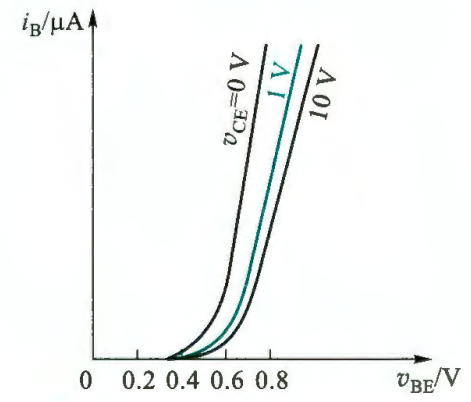
\includegraphics[width=0.35\linewidth]{pic/BJT共射输入特性曲线.png}
    \caption{BJT共射输入特性曲线\cite{康华光}\label{BJT共射输入特性曲线}}
\end{figure}

输入特性曲线如图\ref{BJT共射输入特性曲线}所示。当$v_{\mathrm{CE}}=\qty{0}{V}$时,发射结与集电结并联。

发射结正偏时,输入特性曲线就是PN结正向的伏安特性曲线。同样的$v_{\mathrm{BE}}$下,随着$v_{\mathrm{CE}}$增加,集电极收集载流子能力增加,使得载流子在基区停留时间较短,从而$i_\mathrm{B}$减小,这意味着同样的$v_{\mathrm{BE}}$下$i_\mathrm{B}$更小。

当$v_{\mathrm{CE}}=\qty{1}{V}$时,发射的电子几乎都被集电区收集,电流几乎不再减小。

\subsubsection{二、输出特性曲线:}
输出特性曲线用函数关系表示为:
\begin{equation}
    i_\mathrm{C}=f(v_{\mathrm{CE}})|_{i_{\mathrm{B}}=\mathrm{Const.}}
\end{equation}

\begin{figure}[htb]
    \centering
    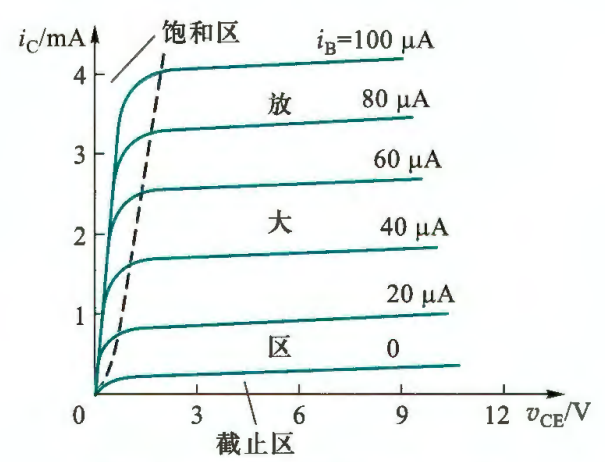
\includegraphics[width=0.45\linewidth]{pic/BJT共射输出特性曲线.png}
    \caption{BJT共射输出特性曲线\cite{康华光}\label{BJT共射输出特性曲线}}
\end{figure}

输出特性曲线的图比输入特性曲线更重要,如图\ref{BJT共射输出特性曲线}所示。可以看出,输出特性曲线分为三个部分:放大区、饱和区和截止区。在模电里,大部分时候BJT只会工作在放大区当放大器件,而在数电里会使BJT工作在饱和区和截止区当开关器件。

当$v_{\mathrm{CE}}=\qty{0}{V}$时,集电结正偏,不能收集载流子,因此$i_{\mathrm{C}}=0$。

1.\textbf{放大区}\index{F!放大区}:工作条件为发射结正偏$v_{\mathrm{BE}}>V_{\mathrm{th}}$、集电结反偏。此时$i_{\mathrm{C}}$受到$i_{\mathrm{B}}$控制,有$i_{\mathrm{C}}=\beta i_{\mathrm{B}}$。

2.\textbf{饱和区}\index{B!(BJT)饱和区}:工作条件为发射结正偏、集电结正偏。此时$v_{\mathrm{CE}}$很小,载流子收集能力较弱。$i_{\mathrm{C}}$几乎不依赖于$i_{\mathrm{B}}$,其中的倾斜主要是因为基区宽度调制效应。此时有$i_{\mathrm{C}}<\beta i_{\mathrm{B}}$。

3.\textbf{截止区}\index{J!截止区}:工作条件为发射结反偏、集电结反偏(准确来说是发射结电压小于开启电压)。BJT无法导通,因此$i_{\mathrm{B}}=0,i_{\mathrm{C}}=I_{\mathrm{CEO}}$。

\section{场效应管(FET)}\index{C!场效应管}
\textbf{场效应管(Field Effect Transistor, FET)},顾名思义,就是利用电场的效应来控制输出电流的一种器件。对于FET,掌握其中的基本概念即可。

FET主要分为两类,结型场效应管\index{C!场效应管!结型场效应管(JFET)}和金属-氧化物-半导体场效应管。与三极管相比,在输出回路输出相同的电流,需要的输入电流的代价更小;同时,因为少子不参与导电,场效应管温度稳定性高,也因此属于\textbf{单极型器件}\index{D!单极型器件}。

\subsection{金属-氧化物-半导体场效应管(MOSFET)}
\textbf{金属-氧化物-半导体场效应管(Metal-Oxide-Semiconductor FET)}\index{C!场效应管!金属-氧化物-半导体场效应管(MOS管)},又称为\textbf{绝缘栅型场效应管}\index{J!绝缘栅型场效应管},或简称为MOS管,目前在大规模集成电路中占据了主导地位。

从载流子的类型来看,分为N沟道MOSFET和P沟道MOSFET;从沟道形成机理来分又各自分为增强型E型(Enhancement)和耗尽型D型(Depletion),将二者两两组合,就形成了四种不同的MOS管。

本节主要讲N沟道增强型MOSFET。

\subsubsection{一、结构}
在低掺杂的P型半导体衬底上生长两个高掺杂的N区,就形成了两个背靠背的PN结,再在衬底上生长一层二氧化硅,并安装三个铝电极,就形成了N沟道增强型MOS管。由制作工艺可以看到其由金属铝、氧化物二氧化硅和半导体硅构成,MOS管也因此得名。

N沟道增强型MOSFET的结构如图\ref{N沟道增强型MOSFET结构}所示,三个区域分别有一些基本特点:

1.\textbf{栅极}\index{S!栅极}g(gate):类比BJT基极b。由于栅极下面有绝缘层二氧化硅,源极、栅极与漏极之间无电接触,有着很高的输入电阻,因此称为“绝缘栅型”场效应管。

2.\textbf{源极}\index{Y!源极}s(source):类比BJT发射极e,提供载流子。

3.\textbf{漏极}\index{L!漏极}d(drain):类比BJT集电极c,载流子流出。一般而言,漏极d与源极s是对称的。但人们往往会将源极s和衬底连接在一起使用,这样栅极和衬底各相当于一个极板,形成电容。当栅-源电压变化时就能改变绝缘层中的感应电荷的多少,从而控制漏极电流。

如图\ref{N沟道增强型MOSFET符号},增强型MOSFET中间为短划线,这意味着$v_{\mathrm{GS}}=0$时沟道断开,而其中箭头指向PN结导通的方向。

\begin{figure}[htb]
    \centering
        \subcaptionbox{N沟道增强型MOSFET结构\cite{康华光}\label{N沟道增强型MOSFET结构}}
        {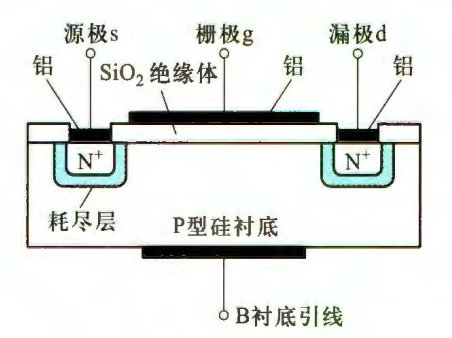
\includegraphics[width=0.45\textwidth]{pic/N沟道增强型MOSFET结构.png}}\qquad
        \subcaptionbox{增强型MOSFET符号\cite{华成英}\label{N沟道增强型MOSFET符号}}
        {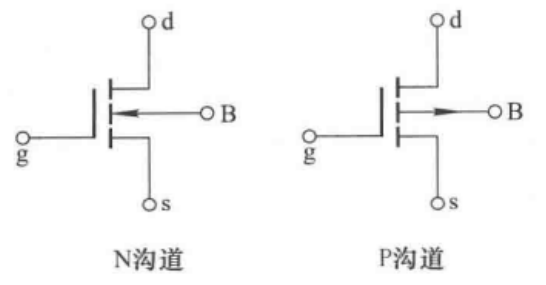
\includegraphics[width=0.45\textwidth]{pic/N沟道增强型MOSFET符号.png}}
        \caption{增强型MOSFET的结构和符号\label{N沟道增强型MOSFET}}
\end{figure}

\subsubsection{二、工作原理}
1.$v_{\mathrm{GS}}=0$,没有\textbf{导电沟道}\index{D!导电沟道},如图\ref{N沟道增强型MOSFET的基本工作原理}(a)所示。即使漏极和源极之间有电压也不会有电流,也因此称为增强型FET。

2.$v_{\mathrm{GS}}\geq V_{\mathrm{TN}}$,出现N型沟道,如图\ref{N沟道增强型MOSFET的基本工作原理}(b)所示。由于绝缘层的存在,不会产生栅极电流,但是会产生指向衬底的强电场,排斥P型衬底中的多子空穴,同时吸引少子自由电子。当$v_{\mathrm{GS}}$大于\textbf{阈值电压}\index{Y!阈值电压}$V_{\mathrm{TN}}$,绝缘层下方形成\textbf{反型层(导电沟道、感生沟道)}\index{F!反型层}。此时N沟道类似于一个被电压控制的可变电阻器,$v_{\mathrm{GS}}$越大,沟道越宽,ds之间的电阻越小。

\begin{figure}[htb]
    \centering
    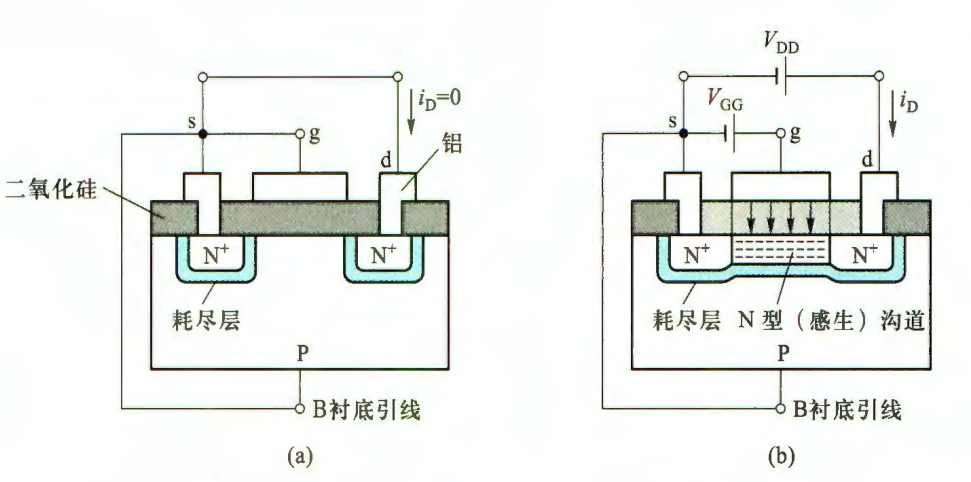
\includegraphics[width=0.65\linewidth]{pic/N沟道增强型MOSFET的基本工作原理.png}
    \caption{N沟道增强型MOSFET的基本工作原理\cite{康华光}\label{N沟道增强型MOSFET的基本工作原理}}
\end{figure}

3.感生沟道出现后,保持$v_{\mathrm{GS}}$不变,施加正的$v_{\mathrm{DS}}$,产生漏极电流$i_{\mathrm{D}}$,同时沟道厚度从左至右不断变薄,如图\ref{可变电阻区和恒流区的形成机制}(a)所示。当$v_{\mathrm{DS}}$较小时,$i_{\mathrm{D}}$与$v_{\mathrm{DS}}$近似线性,此时可等效为\textbf{沟道电阻}\index{G!沟道电阻}。由于$v_{\mathrm{GS}}$可控制沟道电阻大小,因此被称为\textbf{可变电阻区}\index{K!可变电阻区}。

当$v_{\mathrm{DS}}$增大到$v_{\mathrm{DS}}=v_{\mathrm{GS}}-V_{\mathrm{TN}}$时,沟道的漏极侧会被夹断,称为\textbf{预夹断}\index{Y!预夹断},如图\ref{可变电阻区和恒流区的形成机制}(b)所示。若$v_{\mathrm{DS}}$继续增大,由于夹断区电阻远大于沟道其余部分电阻,增加的电压都会落到夹断区,导致其余部分的电压几乎不增加,$i_\mathrm{D}$几乎不随$v_{\mathrm{DS}}$改变,称为\textbf{恒流区}\index{H!恒流区}。

\begin{figure}[htb]
    \centering
    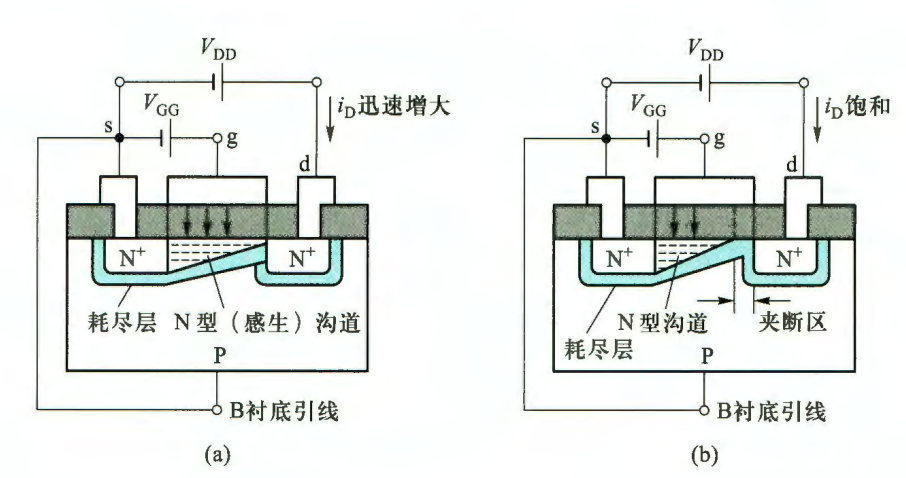
\includegraphics[width=0.65\linewidth]{pic/可变电阻区和恒流区的形成机制.png}
    \caption{可变电阻区和恒流区的形成机制\cite{康华光}\label{可变电阻区和恒流区的形成机制}}
\end{figure}

这样,就得到了一个\textbf{电压控制电流源}——由电压$v_{\mathrm{GS}}$控制的电流$i_\mathrm{D}$。

\subsubsection{三、N沟道耗尽型MOSFET}
\begin{figure}[htb]
    \centering
    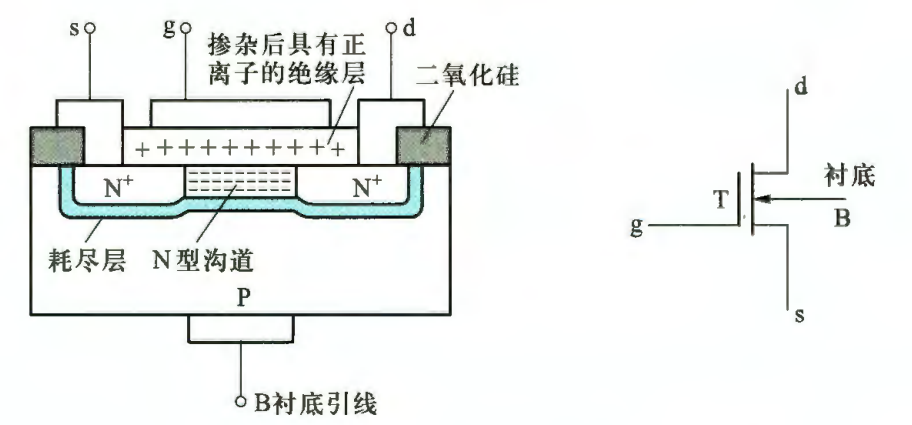
\includegraphics[width=0.6\linewidth]{pic/N沟道耗尽型MOSFET结构和符号.png}
    \caption{N沟道耗尽型MOSFET结构和符号\cite{康华光}\label{N沟道耗尽型MOSFET结构和符号}}
\end{figure}

与增强型不同的是,N沟道耗尽型MOSFET中在二氧化硅绝缘层中加入了大量的正离子(相当于人为先制造一个电场),那么即使$v_{\mathrm{GS}}=0$,也会形成反型层沟道。如图\ref{N沟道耗尽型MOSFET结构和符号}所示,从元件符号来看,ds之间是联通的。

当且仅当$v_{\mathrm{GS}}$为负且达到某一值时,反型层会消失,这个临界值称为\textbf{夹断电压}\index{J!夹断电压}$V_{\mathrm{TN}}$。其余规律和N沟道增强型MOSFET相同。

\subsection{N沟道增强型MOSFET特性曲线}
\subsubsection{一、输出特性曲线}
输出特性曲线的函数关系表示为:
\begin{equation}
    i_\mathrm{D}=f(v_{\mathrm{DS}})|_{v_{\mathrm{GS}}=\mathrm{Const.}}
\end{equation}

\begin{figure}[htb]
    \centering
    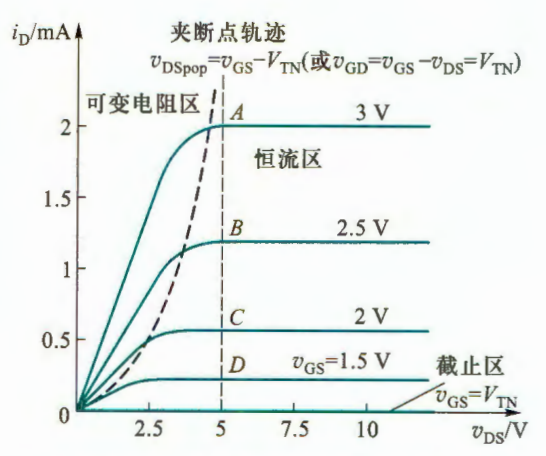
\includegraphics[width=0.45\linewidth]{pic/增强型NMOS管输出特性.png}
    \caption{增强型NMOS管输出特性\cite{康华光}\label{增强型NMOS管输出特性}}
\end{figure}

增强型NMOS管输出特性曲线如图\ref{增强型NMOS管输出特性}所示,与BJT类似,同样可以分为三个区:

1.\textbf{截止区}\index{J!截止区}:当$v_{\mathrm{GS}}<V_{\mathrm{TN}}$时,导电沟道尚未形成,$i_\mathrm{D}=0$。

2.\textbf{可变电阻区}\index{K!可变电阻区}。

3.\textbf{恒流区(放大区)}\index{H!恒流区}。

\subsubsection{二、转移特性}
FET是电压控制器件,由于栅极输入端基本没有电流,故讨论它的输入特性是没有意义的。因此考虑其转移特性曲线,函数关系表示为:

\begin{equation}
    i_\mathrm{D}=f(v_{\mathrm{GS}})|_{v_{\mathrm{DS}}=\mathrm{Const.}}
\end{equation}

\begin{figure}[htb]
    \centering
    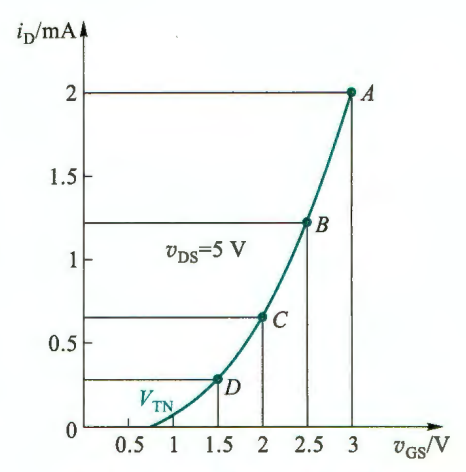
\includegraphics[width=0.35\linewidth]{pic/增强型NMOS管的恒流区转移特性.png}
    \caption{增强型NMOS管的恒流区转移特性\cite{康华光}\label{增强型NMOS管的恒流区转移特性}}
\end{figure}

增强型NMOS管转移特性曲线如图\ref{增强型NMOS管的恒流区转移特性}所示,是一条二次曲线。注意,当工作在恒流区时,才能给出图\ref{增强型NMOS管的恒流区转移特性}。如果是耗尽型,那么只需要将$v_{\mathrm{GS}}$出现的地方做⼀个平移,其他保持不变即可。如果是P沟道,只需要将坐标反向(图像反转180度)。

\subsection{结型场效应管(JFET)}
\textit{(本节的内容仅做了解)}

\textbf{结型场效应管(Junction FET)}\index{C!场效应管!结型场效应管(JFET)}也分为P沟道和N沟道两种类型。由于JFET具体原理与MOS管大同小异,因此不详细展开,本节简单仅讨论N沟道JFET。

\subsubsection{一、结构}
如图\ref{N沟道JFET结构示意图}所示,在同一块N型半导体上制作两个高掺杂的P区,并连接在一起,形成栅极g。N型半导体两端引出两个电极为源极s和漏极d,漏极和源极之间的非耗尽层称为\textbf{导电通道}。

\begin{figure}[htb]
    \centering
    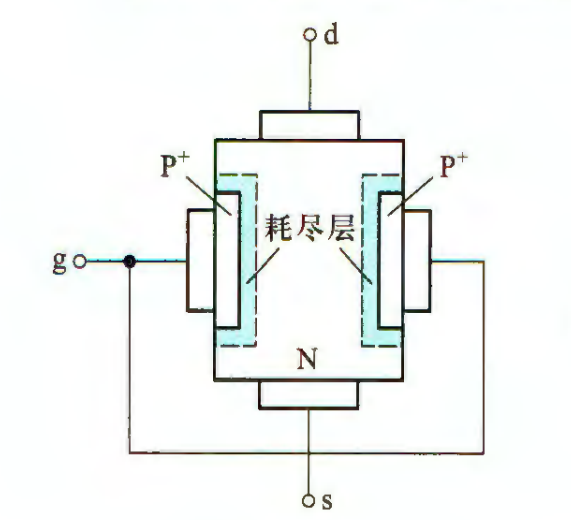
\includegraphics[width=0.35\linewidth]{pic/N沟道JFET结构示意图.png}
    \caption{N沟道JFET结构示意图\cite{康华光}\label{N沟道JFET结构示意图}}
\end{figure}

\subsubsection{二、工作原理}
首先,对于N沟道结型场效应管,当$v_{\mathrm{GS}}>0$时,PN结导通,此时$v_{\mathrm{GS}}$不能实现对沟道电流的控制,因此以下$v_{\mathrm{GS}}$增大全部指的是绝对值增大。

1.$v_{\mathrm{DS}}$,$v_{\mathrm{GS}}$增大时,耗尽层加宽,沟道变窄,沟道电阻增大。当增大到\textbf{夹断电压}$V_\mathrm{P}$时,沟道全部被夹断,沟道电阻变为无穷大。

2.当$V_\mathrm{P}<v_{\mathrm{GS}}<0$时,$v_{\mathrm{DS}}$较小时,由于$v_{\mathrm{GD}}$逐渐减小,靠近漏极的导电沟道逐渐变窄,随后预夹断。此时若$v_{\mathrm{DS}}$继续增大,则耗尽层闭合部分沿着沟道延伸,此时$v_{\mathrm{DS}}$的增大几乎全部用于克服夹断区延伸产生的电阻上,此时$i_\mathrm{D}$恒流。

3.当$v_{\mathrm{DS}}$继续增大时,可能会发生耗尽区击穿(二极管的反向击穿)。